\documentclass[pscyr,titlepage]{hedreport}
\usepackage[russian]{babel}
\usepackage[utf8]{inputenc}
\usepackage{hedmaths}

\usepackage{graphicx}
\graphicspath{{images/}}

\usepackage{color}
\usepackage[colorlinks,linkcolor=black,urlcolor=black]{hyperref}
\renewcommand{\UrlFont}{\rm\small}
\newcommand{\de}{\delta}

\usepackage{setspace}

\newcommand{\eq}[1]{\eqref{eq#1}}
\newcommand{\pic}[1]{\ref{pic#1}}

\faculty{Факультет электроники и вычислительной техники}
\department{физики}
\subject{дисциплине <<Квантовая электроника>>}
\topic{Алгоритмы восстановления формы волнового фронта\\в адаптивных лазерных
  системах}
\student[m]{студент группы Ф-469\\Чечеткин И. А.}
\teacher[m]{к. физ.-мат. наук\\Подопригора А. Г.}

\begin{document}
\maketitle
\onehalfspacing

\section*{Введение}

Оптические элементы, которыми можно управлять, чтобы видоизменить волновой
фронт, называют адаптивной оптикой. Однако не всякие элементы здесь имеются в
виду. Адаптивной традиционную оптику состоящую из линз, зеркал, призм не
считают. Свет от удаленного объекта, проходя через земную атмосферу, испытывает
на своем пути множество преломлений в воздушных потоках. Искажения светового
излучения постоянно сменяют друг друга, по этой причине обычной оптикой
невозможно достичь нужного корректирования волны и соответственно получения
качественного изображения.

Основные задачи, для решения которых создавалась адаптивная оптика это:
\begin{itemize}
  \item наземные телескопы для астрономических исследований;
  \item приемно-передающие информационные лазерные системы, работающие в
    атмосфере;
  \item оптические системы мощных лазеров.
\end{itemize}

Оптическая неоднородность ограничивает когерентность лазерных пучков и не
позволяет достичь требуемой мощности и фокусировки. Этим вызвано широкое
применение оптики, <<умеющей>> уменьшить расходимость лазерных пучков в
атмосфере до дифракционных пределов.Создание адаптивных систем для формирования
лазерных пучков вызвано стремлением уменьшить их расходимость в атмосфере до
дифракционных пределов. Адаптивная оптика позволяет достичь фазировки нескольких
лазерных каналов. Адаптивные оптические системы (\emph{АОС}) незаменимы для
импульсных сигналов, где важнейшей характеристикой адаптивного зеркала является
его возможность отработать необходимую форму волнового фронта за минимальное
время.

В состав типичной АОС, работающей в реальном масштабе времени входят:
\begin{itemize}
  \item Деформируемое зеркало, предназначенное для компенсации искажений
    волнового фронта оптического тракта (разъюстировка оптических элементов и
    погрешности в их изготовлении, влияние турбулентности атмосферы).
  \item Датчик волнового фронта, предназначенный для определения искажений
    волнового фронта. 
  \item Электронные блоки, предназначенные для выработки и передачи управляющих
  команд на исполнительные устройства деформируемого зеркала.
\end{itemize}

\section{Типы адаптивных оптических систем}

На данный момент все адаптивные оптические системы можно разделить на 
основные классы:
\begin{enumerate}
  \item Классические адаптивные системы с прямым измерением волнового
    фронта (с датчиками волнового фронта; системы фазового сопряжения);
  \item Системы, определяющие волновой фронт косвенным образом. В частности, к
    этому классу относится АОС с максимизацией функции резкости. 
\end{enumerate}

\begin{figure}[ht]
  \center
  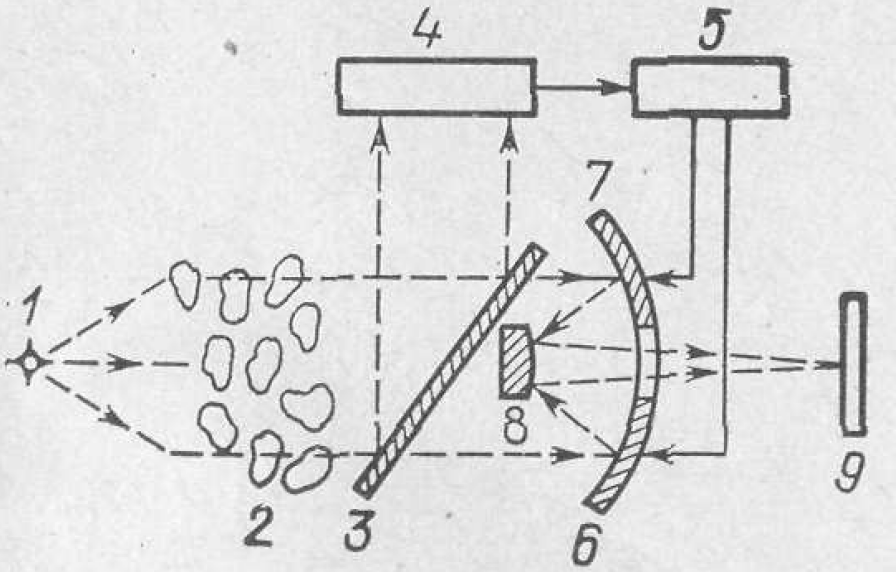
\includegraphics[width=.47\textwidth]{ds_1_1} \hfill
  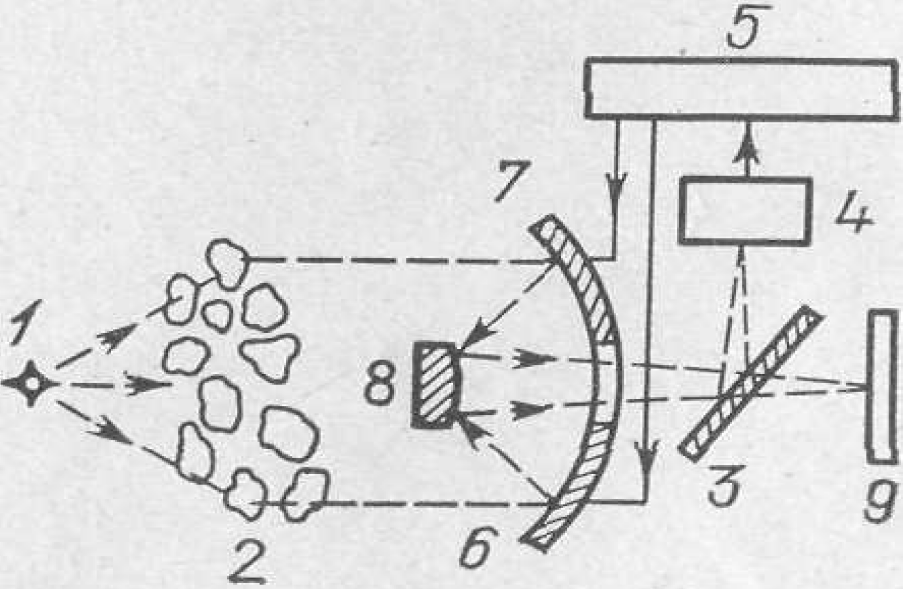
\includegraphics[width=.47\textwidth]{ds_1_2} \\
  \parbox{.47\textwidth}{ \caption{Пример системы прямого управления}
    \label{pic1} } \hfill
  \parbox{.47\textwidth}{ \caption{Пример системы обратного управления}
    \label{pic2} } \\
  {
  \footnotesize
    Свет от звезды 1 проходит через атмосферу 2, искажающую волновой фронт и
    попадает на светоделитель 3. Часть света, отведенная от основного пучка,
    падает на датчик волнового фронта 4, где регистрируется фазовый профиль
    приходящей от объекта волны. На основании этой информации в управляющем
    устройстве 5 вычисляются необходимые координаты управляемых зеркал 6 и 7 и
    формируются соответствующие сигналы управления. Основной пучок света,
    отразившись от зеркал 6, 7 и малого зеркала 8, создает в плоскости 9
    изображение объекта. Датчик 4 расположен до корректирующего элемента,
    и регистрируемая им волна не зависит от работы корректора и системы
    управления. 
  }
\end{figure}

Существуют системы прямого управления (рис.~\pic{1}) и основанные на принципе
обратной связи (рис.~\pic{2}).

Система прямого управления обладает высоким быстродействием, но она не устраняет
искажения вызванные деформацией зеркал телескопа. Так же здесь ошибки
корректирующих элементов не контролируются и соответственно не устраняются. В
системах с обратной связью датчик располагается после корректирующих зеркал.
Всякое искажение волнового фронта независимо от его причины фиксируется датчиком
и вызывает появление управляющих сигналов, стремящихся уменьшить искажения. При
идеальной настройке корректора на датчик должен падать неискаженный волновой
фронт. В такой схеме датчик~-- это индикатор отклонений волнового фронта от его
идеальной формы. Но быстродействие схем с обратной связью заметно меньше.

Возможно создание систем другого типа, где волновой фронт непосредственно вообще
не регистрируется. Для этого в схеме с обратной связью заменяют датчик
устройством, измеряющим только интенсивность в центре дифракционного максимума
изображения точечного объекта. Эта интенсивность играет роль целевой функции
(критерий качества). Организовывают процесс управления в системе так, чтобы
максимизировать эту функцию. При апертурном зондировании субапертурам сообщают
пробные движения и, наблюдая за изменением целевой функции, определяют
необходимое направление движения корректора. Во многих случаях результатом
действия систем апертурного зондирования является формирование фазосопряженного
сигнала \( e^{-iS} \) уходящего к цели.

Подходом, известным ранее, как апертурное зондирование или технология
максимизации функции резкости изображений, а в настоящее время известным, как
управление волновым фронтом (\emph{ВФ}) на основе оптимизаций функций качества
градиентными методами, долгое время пренебрегали (из-за медленной работы таких
систем). Несколько факторов вносят вклад в возрождение метода свободной
оптимизации в адаптивной оптике:
\begin{enumerate}
  \item Трудности, связанные с использованием методов прямого измерения ВФ при
    наличии сильных флуктуаций интенсивности, стимулировали поиск новых типов
    адаптивных систем.
  \item Для некоторых приложений адаптивной оптики, таких как анизопланатизм,
    лазерное формирование изображений и фокусировка лазерного излучения через
    фазоискажающие среды на протяженные объекты, наземная лазерная связь и т.~д.,
    АОС с прямым измерением ВФ не могут быть использованы без привлечения
    технологий <<лазерной звезды>>.
  \item Появление недорогих адаптивных корректоров на базе
    микроэлектромеханических систем и жидкокристаллических фазовых модуляторов
    создают хорошую основу для разработки современных быстродействующих,
    небольших по габаритам и недорогих АОС. Однако достижению этой цели мешает
    отсутствие эффективных датчиков волнового фронта (\emph{ДВФ}).
  \item Разрабатываемые в последние годы новые параллельные алгоритмы
    оптимизации на основе математических методов стохастической аппроксимации и
    их программно-аппаратная реализация в виде больших интегральных систем
    позволят создавать эффективные быстродействующие средства цифровой обработки
    сигналов и изображений, которые успешно могут быть использованы в адаптивной
    оптике.
\end{enumerate}

Пробные возмущения могут вносится последовательно для каждого участка коррекции
ВФ и параллельно для всех участков сразу. Метод измерения градиентных компонент
основывается на вычислении точного градиента внесением малых возмущений 
\( \de u_j \) в одно время и измерением ответного изменения \( \de J_j \)
величины качества отображения. Отношения \( \de J_j / \de u_j \)
используются как аппроксимации для точного значения градиента компонент. Для
полного определения точного градиента требуется \( N \) последующих возмущений
со временными потерями возрастающими с возрастанием числа каналов управления
\( N \).

\section{Аппроксимация градиента, его оценка на основе параллельной
стохастической аппроксимации}

Градиентный метод минимизации целевой функции \( J[\phi] \) сводится к движению
точки \( \phi \), соответствующей корректирующей фазе, в некотором пространстве
оптимизации под действием <<силы>>, направленной в сторону антиградиента или в
направлении, противоположном  первой  вариации  функционала \( J[\phi] \).
Движение точки в этом случае описывается дифференциальным уравнением
\begin{equation}
  \tau\pder{\phi(\vec{r}, t)}{t} = -\de_\phi J[\phi(\vec{r}, t)],
  \label{eq1}
\end{equation}
где \( \tau \)~-- временная постоянная, \( \de_\phi \)~-- вариация.
Траектория движения \( \phi(\vec{r}, t) \), определяемая этим уравнением,
приводит к экстремальной точке. В адаптивной оптике зависимость \( J[\phi] \) и
модель системы, которая может включать в себя искажения ВФ в турбулентной
атмосфере, в общем случае являются неизвестными (т.~н. <<слепая модель>> или
<<слепая адаптация>>) и вариация \( \de_\phi J[\phi] \) должна быть
определена на основе измеренных данных \( J[\phi] \).

Размерность процесса \eq{1} может быть уменьшена путем представления
корректирующего ВФ \( \phi(\vec{r}, t) \), в следующем виде
\[
  \phi(\vec{r}, t) = \sum_{j = 1}^N u_j(\vec{r}, t) S_j(\vec{r}),
\]
где \( u_j(\vec{r}, t) \)~-- управляющий сигнал, описывающий напряжение,
прилагаемое к \( j \)-му электроду корректора (адаптивного зеркала), а
\( S_j \)~-- соответствующая функция отклика. Тогда вместо выражения \eq{1}
имеем систему обыкновенных дифференциальных уравнений, описывающих изменение
управляющих сигналов в процессе адаптации
\begin{equation}
  \tau_j \pder{u_j(\vec{r}, t)}{t} = -\gamma J_j'(u_1, \ldots, u_N),
  \label{eq3}
\end{equation}
где \( \tau_j \)~-- временные постоянные, а
\( J_j' = \pder{J(u_1, \ldots, u_N)}{u_j} \)~-- \( j \)-я компонента градиента
целевой функции \( J(u_1, \ldots, u_N) \). Здесь коэффициент \( \gamma \)
положителен при минимизации \( J \) и отрицателен в противном случае.

Для дискретного процесса \( \{ t_n, n=1,\ldots \} \) выражение \eq{3}
записывается в виде
\begin{equation}
  u_j^{(n+1)} = u_j^{(n)} - \gamma J_j'(u_1^(n), \ldots, u_N^{(n)}), \quad
    j = 1, \ldots, N.
  \label{eq5}
\end{equation}

В основе метода параллельной стохастической аппроксимации (\emph{ПСА}) градиента
лежит следующая идея: пусть небольшие возмущения управляющих сигналов
\( \{ \de u_j, j = 1, \ldots, N \} \) вводятся во всех каналах одновременно
(параллельно). Тогда изменение целевой функции \( \de J \)
\[
  \de J = J(u_1 + \de u_1, \ldots, u_j + \de u_j, \ldots u_N + \de u_N) -
    J(u_1, \ldots, u_j, \ldots, u_N)
\]
можно представить в виде разложения в ряд Тейлора
\begin{equation}
  \de J = \sum_{j = 1}^N \pder{J}{u_j}\de u_j + \frac{1}{2}\sum_{j,k = 1}^N
    \pcder{J}{u_j}{u_k}\de u_j \de u_k + \ldots,
  \label{eq9}
\end{equation}
откуда следует выражение
\begin{equation}
  \de J\de u_j = \pder{J}{u_j}(\de u_j)^2 + \psi_j, \text{ где }
    \psi_j = \sum_{\begin{smallmatrix} k = 1, \\ k\ne j \end{smallmatrix}}^N
    \pder{J}{u_k} \de u_j\de u_k + \frac{1}{2} \sum_{k, l = 1}^N
    \pcder{J}{u_k}{u_l} \de u_j\de u_k\de u_l + \ldots,
  \label{eq10}
\end{equation}
которое и является исходным для нахождения оценок компонентов градиента.

Выражение \eq{9} является наиболее общей записью изменения целевой функции
\( \de J \). Чтобы обеспечить более точную оценку градиента \( J_j' \),
амплитуда второго члена в \eq{10} должна быть малой. Исходя из этого, основное
различие между методами оценки градиента состоит в способах ограничения второго
члена. В методе последовательных возмущений второй член равен нулю, как
результат выполнения последовательных событий, для которых \( \de u_j \ne 0 \)
только тогда, когда \( \de u_k = 0 \) для всех \( k \ne j \). В методе
многоканальной фазовой модуляции второй член содержит только гармонические
компоненты (суммарные или разностные), которые при правильно выбранном диапазоне
частот модуляции фильтруются синхронными детекторами.

В методе ПСА, если вводимые возмущения являются случайными и статистически
независимыми, то второй член в выражении \eq{10} уменьшается до нуля (в среднем)
и оценка градиента \( J_j' \approx \de J\de u_j \) (величина случайная) является
состоятельной и несмещенной. Таким образом, аппроксимация
\[
  \pder{J}{\phi_j} = J_j' \approx \frac{\de J\cdot\de\phi_j}{\sigma_\phi^2},
\]
где \( \{ \de\phi_j, j = 1,\ldots, N \} \)~-- статистически независимые
случайные возмущения в каждом канале фазового корректора (адаптивного зеркала),
имеющие нормальное распределение с нулевым средним и дисперсией
\( \sigma_\phi^2 \), может быть непосредственно использована, как оценка градиента в 
непрерывном \eq{3} или дискретном \eq{5} виде. 

Одной из наиболее распространенных функций качества АОС (целевой функцией)
является резкость изображений \( J \), которая записывается в виде
\begin{equation}
  J = \int I^2(\vec{r})\,d\vec{r},
  \label{eq11}
\end{equation}
где \( I(\vec{r}) \)~-- интенсивность изображения в фокусе приемной оптической
системы. Её широкое использование в АОС обусловлено наличием однозначной связи
между глобальным максимумом \( J \) и полной компенсацией атмосферных фазовых
искажений.

\pagebreak % -------------------------------------------------------------------
\renewcommand{\bibname}{Список литературы}

\begin{thebibliography}{9}
  \bibitem{1} Ермолаева, Е.~В., Зверев, В.~А., Филатов, А.~А. Адаптивная
    оптика~/\\ Е.~В. Ермолаева, В.~А. Зверев, А.~А. Филатов~-- СПб.: НИУ
    ИТМО,~2012.~-- 297~с.
  \bibitem{2} Польских, С.~Д. Восстановление оптических изображений космических
    объектов, искаженных турбулентной атмосферой~/ Лазерно-оптические системы и
    технологии~-- М.: ФГУП <<НПО Астрофизика>>,~2009.~-- С.~41.
  \bibitem{3} О принципиальной возможности уменьшения влияния атмосферы на
    изображение звезды. Опт. и спектр., т. 3, вып. 4~-- 1957.~-- С.~401--402.
\end{thebibliography}

\end{document}